% **************************************************************************************************************
% A Classic Thesis Style
% An Homage to The Elements of Typographic Style
%
% Copyright (C) 2010 André Miede http://www.miede.de
%
% If you like the style then I would appreciate a postcard. My address
% can be found in the file ClassicThesis.pdf. A collection of the
% postcards I received so far is available online at
% http://postcards.miede.de
%
% License:
% This program is free software; you can redistribute it and/or modify
% it under the terms of the GNU General Public License as published by
% the Free Software Foundation; either version 2 of the License, or
% (at your option) any later version.
%
% This program is distributed in the hope that it will be useful,
% but WITHOUT ANY WARRANTY; without even the implied warranty of
% MERCHANTABILITY or FITNESS FOR A PARTICULAR PURPOSE.  See the
% GNU General Public License for more details.
%
% You should have received a copy of the GNU General Public License
% along with this program; see the file COPYING.  If not, write to
% the Free Software Foundation, Inc., 59 Temple Place - Suite 330,
% Boston, MA 02111-1307, USA.
%
% **************************************************************************************************************
% Note:
%    * You must not use "u etc. in strings/commands that will be spaced out (use \"u or real umlauts instead)
%    * New enumeration (small caps): \begin{aenumerate} \end{aenumerate}
%    * For margin notes: \graffito{}
%    * Do not use bold fonts in this style, it is designed around them
%    * Use tables as in the examples
%    * See classicthesis-ldpkg.sty for useful commands
% **************************************************************************************************************
% To Do:
%		 * [high] Check this out: http://www.golatex.de/koma-script-warnung-in-verbindung-mit-listings-package-t2058.html
%    * [medium] mathbb in section-titles/chapter-titles => disappears somehow in headlines!!!
%    * [low] Calculate text block size for Libertine font
%    * [low] Think about processing a4paper, a5paper, 10pt, 11pt, 12pt etc. options for typearea layout
%            (store values in internal variables and handle by \AtEndOfPackage{\areaset...})
% **************************************************************************************************************
\documentclass[ oneside,openright,titlepage,fleqn,numbers=noenddot,headinclude,%1headlines,%
                11pt,a4paper,BCOR5mm,footinclude,cleardoublepage=empty,abstractoff % <--- obsolete, remove (todo)
                ]{scrreprt}

% ********************************************************************
% Development Stuff
% ********************************************************************
\listfiles
%\usepackage[l2tabu, orthodox, abort]{nag}
%\usepackage[warning, all]{onlyamsmath}
% ********************************************************************
% Re-usable information
% ********************************************************************
\usepackage[utf8x]{inputenc}
\newcommand{\myTitle}{Operating Systems Imaging Solution with Centralised Archiving and Distribution\xspace}
\newcommand{\myDegree}{Bachelor Thesis\xspace}
\newcommand{\myName}{Alexandru Juncu\xspace}
\newcommand{\myProf}{Conf. Dr. Ing. Răzvan Rughiniș\xspace}
%\newcommand{\myOtherProf}{Put name here\xspace}
%\newcommand{\mySupervisor}{Put name here\xspace}
\newcommand{\myFaculty}{Automatic Control and Computer Science Faculty\xspace}
\newcommand{\myDepartment}{Computer Science and Engineering Department\xspace}
\newcommand{\myUni}{\protect{University \emph{Politehnica} of Bucharest}\xspace}
\newcommand{\myLocation}{Bucharest\xspace}
\newcommand{\myTime}{July 2010\xspace}
\newcommand{\myVersion}{Version 1.0\xspace}


%*******************************************************
% Packages with options that might require adjustments
%*******************************************************
\usepackage[american]{babel}
\usepackage[square,numbers]{natbib}
\usepackage[fleqn]{amsmath} % math environments and more by the AMS

%*******************************************************
\usepackage{classicthesis-ldpkg} % [backref]
%*******************************************************
% Options for classicthesis.sty:
% tocaligned eulerchapternumbers rafting linedheaders listsseparated
% subfig nochapters beramono eulermath parts minionpro pdfspacing
% listings dottedtoc minionprospacing manychapters
\usepackage[eulerchapternumbers,listings,listsseparated,%pdfspacing,%listings,
						subfig,beramono,eulermath,parts]{classicthesis}

%*******************************************************
% Some font experiments
%*******************************************************
%\usepackage[osf]{libertine}
%\usepackage{hfoldsty}
%\usepackage[light,condensed,math]{iwona}
%\renewcommand{\sfdefault}{iwona}
%\usepackage{lmodern} % <-- no osf support :-(
%\usepackage[urw-garamond]{mathdesign} <-- no osf support :-(

%*******************************************************
% Fine-tuning for the text area
%*******************************************************
%\linespread{1.05} % a bit more for Palatino
%\areaset[5mm]{312pt}{761pt} % 686 (factor 2.2) + 33 head + 42 head \the\footskip
%\setlength{\marginparwidth}{7em}%
%\setlength{\marginparsep}{2em}%

%*******************************************************
% hack to use citations in float environments
% will be fixed with caption package version 3.2
%*******************************************************

%%%%%bug
\usepackage{makerobust}
\makeatletter
\MakeRobustCommand\caption@xref
\makeatother

%*******************************************************
%\usepackage[section,below]{placeins} <--- not everybody wants this
%\usepackage[all]{hypcap} <--- does not work with MiKTeX 2.6
% ********************************************************************
% Language/strings for backrefs (change here, thanks, Lorenzo)
%*******************************************************
%\renewcommand{\backrefnotcitedstring}{\relax}%(Not cited.)
%\renewcommand{\backrefcitedsinglestring}[1]{(Citato a pagina~#1.)}
%\renewcommand{\backrefcitedmultistring}[1]{(Citato alle pagine~#1.)}
%\renewcommand{\backreftwosep}{ e~}
%\renewcommand{\backreflastsep}{ e~}
% ********************************************************************
% Setup and Finetuning
%*******************************************************
\newlength{\abcd} % for ab..z string length calculation
\newcommand{\myfloatalign}{\centering} % how all the floats will be aligned
\setlength{\extrarowheight}{3pt} % increase table row height
% ********************************************************************
% Captions look and feel
%*******************************************************
\captionsetup{format=hang,font=small}
% ********************************************************************
% Listings setup
% ********************************************************************
%\lstset{emph={trueIndex,root},emphstyle=\color{BlueViolet}}%\underbar} % for special keywords
% ********************************************************************
\lstset{language=[LaTeX]Tex,%C++,
    keywordstyle=\color{RoyalBlue},%\bfseries,
    basicstyle=\small\ttfamily,
    %identifierstyle=\color{NavyBlue},
    commentstyle=\color{Green}\ttfamily,
    stringstyle=\rmfamily,
    numbers=none,%left,%
    numberstyle=\scriptsize,%\tiny
    stepnumber=5,
    numbersep=8pt,
    showstringspaces=false,
    breaklines=true,
    frameround=ftff,
    frame=single,
    belowcaptionskip=.75\baselineskip,
    numberbychapter=false
    %frame=L
}

% ********************************************************************
% Where to look for graphics
%*******************************************************
%\graphicspath{{gfx/}{misc/}} % considered harmful according to l2tabu
% ********************************************************************
% Hyperreferences
%*******************************************************
\hypersetup{%
    colorlinks=true, linktocpage=true, pdfstartpage=3, pdfstartview=FitV,%
    % uncomment the following line if you want to have black links (e.g., for printing)
    %colorlinks=false, linktocpage=false, pdfborder={0 0 0}, pdfstartpage=3, pdfstartview=FitV,%
    breaklinks=true, pdfpagemode=UseNone, pageanchor=true, pdfpagemode=UseOutlines,%
    plainpages=false, bookmarksnumbered, bookmarksopen=true, bookmarksopenlevel=1,%
    hypertexnames=true, pdfhighlight=/O,%hyperfootnotes=true,%nesting=true,%frenchlinks,%
    urlcolor=webbrown, linkcolor=RoyalBlue, citecolor=webgreen, %pagecolor=RoyalBlue,%
    %urlcolor=Black, linkcolor=Black, citecolor=Black, %pagecolor=Black,%
    pdftitle={\myTitle},%
    pdfauthor={\textcopyright\ \myName, \myUni, \myFaculty},%
    pdfsubject={},%
    pdfkeywords={},%
    pdfcreator={pdfLaTeX},%
    pdfproducer={LaTeX with hyperref and classicthesis}%
}

%********************************************************************
% Hyphenation
%*******************************************************
%\hyphenation{put special hyphenation here}
% ********************************************************************
% GO!GO!GO! MOVE IT!
%*******************************************************
\begin{document}
\frenchspacing
\raggedbottom
\selectlanguage{american} % american ngerman
%\renewcommand*{\bibname}{new name}
%\setbibpreamble{}
\pagenumbering{roman}
\pagestyle{plain}
%********************************************************************
% Frontmatter
%*******************************************************
%%*******************************************************
% Little Dirty Titlepage
%*******************************************************
\thispagestyle{empty}
%\pdfbookmark[1]{Titel}{title}
%*******************************************************
\begin{center}
    \spacedlowsmallcaps{\myName} \\ \medskip

    \begingroup
        \color{Maroon}\spacedallcaps{\myTitle}
    \endgroup
\end{center}

%*******************************************************
% Titlepage
%*******************************************************
\begin{titlepage}
  % if you want the titlepage to be centered, uncomment and fine-tune the line below (KOMA classes environment)
  \begin{addmargin}[-1cm]{-3cm}
    \begin{center}
        \large

        \hfill

        \vfill

        \begingroup
            \color{Maroon}\spacedallcaps{\myTitle} \\ \bigskip
        \endgroup

        \spacedlowsmallcaps{\myName}

        \vfill

        
\includegraphics[width=6cm]{gfx/cs} \\ \medskip

        \myDegree \\ \medskip
        \myDepartment \\
        \myFaculty \\
        \myUni \\ \bigskip

        \myTime

        \vfill

    \end{center}
  \end{addmargin}
\end{titlepage}

\thispagestyle{empty}

\hfill

\vfill

\noindent\myName: \textit{\myTitle,} \myDegree, \textcopyright\ \myTime

\bigskip

\noindent\spacedlowsmallcaps{Supervisors}: \\
\myProf \\
%\myOtherProf %\\
%\mySupervisor

\medskip

\noindent\spacedlowsmallcaps{Location}: \\
\myLocation

\medskip

\noindent\spacedlowsmallcaps{Time Frame}: \\
\myTime

%\cleardoublepage%*******************************************************
% Dedication
%*******************************************************
\thispagestyle{empty}
%\phantomsection
\refstepcounter{dummy}
\pdfbookmark[1]{Dedication}{Dedication}

\vspace*{3cm}

\begin{center}
    \emph{Ohana} means family. \\
    Family means nobody gets left behind, or forgotten. \\ \medskip
    --- Lilo \& Stitch
\end{center}

\medskip

\begin{center}
    Dedicated to the loving memory of Rudolf Miede. \\ \smallskip
    1939\,--\,2005
\end{center}

\cleardoublepage%*******************************************************
% Abstract
%*******************************************************
%\renewcommand{\abstractname}{Abstract}
\pdfbookmark[1]{Abstract}{Abstract}
\begingroup
\let\clearpage\relax
\let\cleardoublepage\relax
\let\cleardoublepage\relax

\chapter*{Abstract}
This thesis presents an advanced imaging solution for Operating System
Multiplication over the network based on UDP Cast with a suite of added
software. It presents the idea for a centralized archiving system and
distribution of the images over the network along with the deployment
of the solution.

The fist chapters present the features of UDP Cast, an open source project
for multicast transmission of data, along with the shortcomings of
UDP Cast.

The proposed project in the thesis focuses on implementing a system that
fixes the discovered problems. The idea presented is an architecture with
an Imaging Client and an Imaging Server.

The last chapters present the implementation of the Client and the Server,
ending with the evaluation on the model.



\endgroup

\vfill

%\cleardoublepage%*******************************************************
% Publications
%*******************************************************
\pdfbookmark[1]{Publications}{publications}
\chapter*{Publications}
Some ideas and figures have appeared previously in the following publications:

\bigskip

\noindent Put your publications from the thesis here.
%\cleardoublepage%*******************************************************
% Acknowledgments
%*******************************************************
\pdfbookmark[1]{Acknowledgments}{acknowledgments}

\begin{flushright}{\slshape
    We have seen that computer programming is an art, \\
    because it applies accumulated knowledge to the world, \\
    because it requires skill and ingenuity, and especially \\
    because it produces objects of beauty.} \\ \medskip
    --- \defcitealias{knuth:1974}{Donald E. Knuth}\citetalias{knuth:1974} \citep{knuth:1974}
\end{flushright}



\bigskip

\begingroup
\let\clearpage\relax
\let\cleardoublepage\relax
\let\cleardoublepage\relax
\chapter*{Acknowledgments}
Put your acknowledgments here.

Many thanks to everybody who already sent me a postcard!

Regarding the typography and other help, many thanks go to Marco 
Kuhlmann, Philipp Lehman, Lothar Schlesier, Jim Young, Lorenzo 
Pantieri and Enrico Gregorio\footnote{Members of GuIT (Gruppo 
Italiano Utilizzatori di \TeX\ e \LaTeX )}, J\"org Sommer, 
Joachim K\"ostler, Daniel Gottschlag, Denis Aydin, Paride 
Legovini, Steffen Prochnow, Nicolas Repp, Hinrich Harms, 
and the whole \LaTeX-community for support, ideas and some great software.

\endgroup




\pagestyle{scrheadings}
\cleardoublepage%*******************************************************
% Table of Contents
%*******************************************************
%\phantomsection
\refstepcounter{dummy}
\pdfbookmark[1]{\contentsname}{tableofcontents}
\setcounter{tocdepth}{2} % <-- 2 includes up to subsections in the ToC
\setcounter{secnumdepth}{3} % <-- 3 numbers up to subsubsections
\manualmark
\markboth{\spacedlowsmallcaps{\contentsname}}{\spacedlowsmallcaps{\contentsname}}
\tableofcontents 
\automark[section]{chapter}
\renewcommand{\chaptermark}[1]{\markboth{\spacedlowsmallcaps{#1}}{\spacedlowsmallcaps{#1}}}
\renewcommand{\sectionmark}[1]{\markright{\thesection\enspace\spacedlowsmallcaps{#1}}}%*******************************************************
% List of Figures and of the Tables
%*******************************************************
\clearpage

\begingroup
    \let\clearpage\relax
    \let\cleardoublepage\relax
    \let\cleardoublepage\relax
    %*******************************************************
    % List of Figures
    %*******************************************************    
    %\phantomsection
    \refstepcounter{dummy}
    %\addcontentsline{toc}{chapter}{\listfigurename}
    \pdfbookmark[1]{\listfigurename}{lof}
    \listoffigures

    \vspace*{8ex}

    %*******************************************************
    % List of Tables
    %*******************************************************
    %\phantomsection
    \refstepcounter{dummy}
    %\addcontentsline{toc}{chapter}{\listtablename}
    \pdfbookmark[1]{\listtablename}{lot}
    \listoftables

    \vspace*{8ex}
%   \newpage

    %*******************************************************
    % List of Listings
    %*******************************************************      
    %\phantomsection
    \refstepcounter{dummy}
    %\addcontentsline{toc}{chapter}{\lstlistlistingname}
    \pdfbookmark[1]{\lstlistlistingname}{lol}
    \lstlistoflistings

    \vspace*{8ex}

    %*******************************************************
    % Acronyms
    %*******************************************************
    %\phantomsection
    \refstepcounter{dummy}
    \pdfbookmark[1]{Acronyms}{acronyms}
    \markboth{\spacedlowsmallcaps{Acronyms}}{\spacedlowsmallcaps{Acronyms}}
    \chapter*{Acronyms}
    \begin{acronym}[UML]
        \acro{API}{Application Programming Interface}
        \acro{UML}{Unified Modeling Language}
        \acro{OS}{Operating System}
        \acro{GUI}{Graphical User Interface}
	\acro{CLI}{Command Line Interface}
	\acro{IP}{Internet Protocol}
	\acro{UDP}{User Datagram Protocol}
	\acro{TCP}{Transmission Control Protocol}
	\acro{PXE}{Preboot Execution Environment}
	\acro{DHCP}{Dynamic Host Configuration Protocol}
	\acro{TFTP}{Trivial File Transfer Protocol}
	\acro{TTL}{Time To Live}
	\acro{GZIP}{GNU zip}
	\acro{LZOP}{Lempel-Ziv-Oberhumer compresion}
	\acro{PIM}{Protocol Independent Multicast}
	\acro{IGMP}{Internet Group Management Protocol}
	\acro{IANA}{Internet Assigned Numbers Authority}
	\acro{MBR}{Master Boot Record}
	\acro{GPL}{Generic Public License}
	\acro{LAN}{Local Area Network}
	\acro{NIC}{Network Interface Card}
	\acro{HDD}{Hard Disk Drive}
	\acro{NTP}{Network Time Protocol}
	\acro{AS}{Autonomous System}
	\acro{RPF}{Reverse Path Forwarding}
	\acro{BIOS}{Basic Input Output System}

    \end{acronym}
\endgroup

\cleardoublepage

%********************************************************************
% Mainmatter
%*******************************************************
\pagenumbering{arabic}
% use \cleardoublepage here to avoid problems with pdfbookmark
%\cleardoublepage\part{Some Kind of Manual}


\chapter{Introduction}\label{ch:intro}
\bigskip



\section{Purpose of the Project}

The \emph{OS Imaging System with Centralised Archiving and Distribution}
is an open source project based on open source tools made for the purpose
of optimising the imaging operations in environments such as school or
university laboratory with a network of workstations. It is built around
frameworks such as UDP Cast, an open source tool for system imaging and
Python, a popular programming language with many libraries  available.

The project plans to introduce features to the normal idea of an imaging
system, such as the possibility to archive and backup Operating System
Images and, most important, provide an always-available server with a
database of images.

The network infrastructure is built upon the Multicast protocol in IP.
This is used to optimise the traffic in the network by reducing the number
of unicast streams in the client-server model to a single multicast stream.

\section{The need for imaging systems}


Setting up a computer means two things: getting the hardware (a normal
PC) and installing a modern Operating System on it to control that
hardware. This is a job that would take a normal person, with basic
computer operating skills, about one hour on average. However, the
normal approach does not scale to installing on 3 or more hosts that
need the exact same setup.


In office environments, Internet/Game Cafes and, most important, in
school laboratories where 15 to 20 computers with identical
configuration need to be set up, an imaging solution is needed.  This
means that the setup will be done on a single computer and then, the
entire disk on which the new operating system resides is copied
throughout the network onto the disks of the other uninstalled hosts.
This can save, for a number of 20 hosts, from 20 hours of work to only
two hours (about one hour for installing one system and another hour
for the copy of the disk(s) over the network).


To get a perfect mirroring, it is recommended that the hosts be
identical (same CPU, same Main board, same \ac{HDD}s, same network card).
If the systems differ in a slight way, it is up to the operating
system to try and adapt to new hardware and install the appropriate
drivers.  From the operating system’s point of view, it is like the
HDD was taken out of one computer and installed in another one.

\begin{figure}[h]
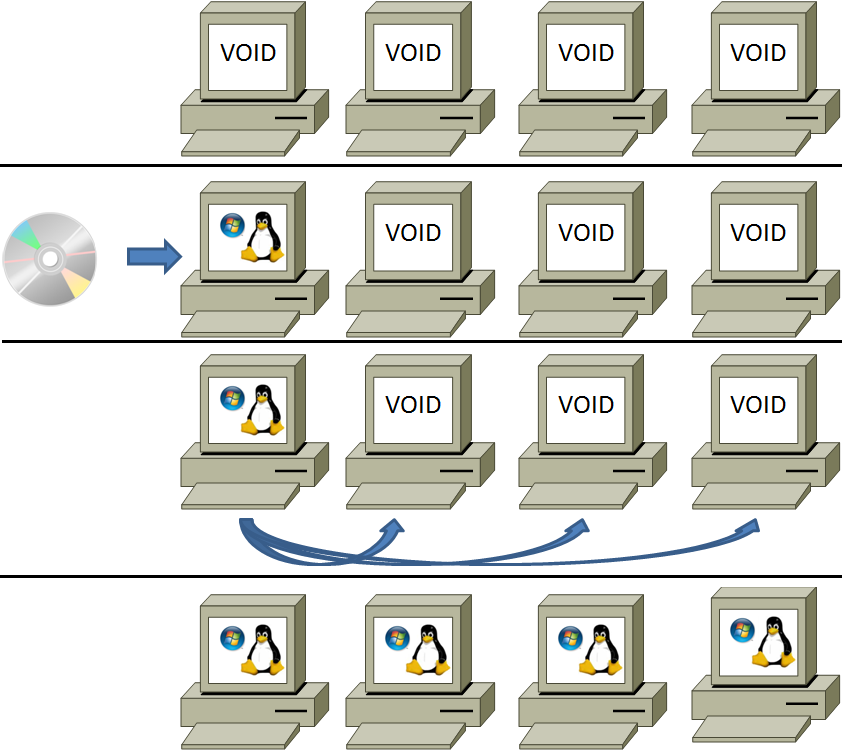
\includegraphics[width=10cm]{img/4comp}
\caption{Simple imaging operations}
\label{fig:4comp}
\end{figure}


To image a network of stations, there are some basic steps you need to take

\begin{enumerate}
\setcounter{enumi}{0}
\item Prepare all the hosts so they can power on. They can have empty
hard disks or hard disks with data that can be deleted.


\item Install one or more operating systems on one host.  This host will
be the seed host.  The operating system(s) can be personalized with
user accounts, installed programs, configured environments. Along with
the operating system(s), on the hard disk there will be the stage 1
boot loader in the \ac{MBR} and the upper stages of the boot loader on
other partitions. Separate partitions for personal data or backups can
be created


\item All the hosts must be able to boot in a pseudo-operating system
provided by the imaging software from a Live CD,  over the network via
PXE or from a local special partition so the working operating is not
modified during the imaging operation.


\item The contents of the seed’s hard disk are copied over the network
(usually using UDP over Multicast IP).  After the transfer is
complete, all hosts boot up normally.
\end{enumerate}



When using imaging systems, software licensing must be taken under
consideration.  The software that has per host or per CPU license has
to have a separate license code for each host.
There are two widely used software suits that provide system imaging:
Symatec Norton Ghost and UDP Cast. The first one is a professional
closed source enterprise software while the second one is an open
source project developed by a community.  Because of the flexibility
of open source projects, UDP cast, has been used in the development of
this imaging system solution and will be described in more detail.





\chapter{Technologies Used}\label{ch:tech}
\bigskip

\section{UDP Cast}

UDP Cast is an open source project that offers a file transfer tool
that can send data simultaneously to many destinations on a \ac{LAN}, under
the \ac{GPL} 2.0 License. The program, along with its source code can be
downloaded from their site, at http://udpcast.linux.lu/.
The compiled projects, offers two executables:  udp-sender and
udp-receiver. By default, the two programs can be used to send input
from standard input on the sever side to all the clients which print
the received data to standard output.

\begin{lstlisting}[caption=Simple udp-sender running]
alexj@lucy:~$ udp-sender
Udp-sender 2004-05-31
Using mcast address 232.168.230.160
UDP sender for (stdin) at 192.168.230.160 on eth0 
Broadcasting control to 192.168.230.255
New connection from 192.168.230.160  (#0) 00000019
Ready. Press any key to start sending data.
Starting transfer: 00000019
Hello
This is a test for the UDP Cast sender & receiver program
bytes= 64 re-xmits=000000 (  0.0%) slice=0162  73 709 551 615 -   0
Transfer complete.
Disconnecting #0 (192.168.230.160)

\end{lstlisting}

\begin{lstlisting}[caption=Simple udp-receiver running]
alexj@lucy:~$ udp-receiver
Udp-receiver 2004-05-31
UDP receiver for (stdout) at 192.168.230.160 on eth0
received message, cap=00000019
Connected as #0 to 192.168.230.160
Listening to multicast on 232.168.230.160
Press any key to start receiving data!
Hello=             64  (  0.71 Mbps) 73 709 551 615 
This is a test for the UDP Cast sender & receiver program
bytes=             64  (  0.00 Mbps) 73 709 551 615 
Transfer complete.
\end{lstlisting}


Using the two simple programs, a file can be transfered to multiple clients
in a single transfer.





\begin{lstlisting}[float,caption=File transfer from a server to two clients]
SERVER:

alexj@hera:~$ cat my_file 
This file has some content.
alexj@hera:~$ udp-sender --file my_file 
Udp-sender 2004-05-31
Using mcast address 232.168.230.160
UDP sender for my_file at 192.168.230.160 on eth0 
Broadcasting control to 192.168.230.255
New connection from 192.168.230.160  (#0) 00000019
Ready. Press any key to start sending data.
New connection from 192.168.230.129  (#1) 00000019
Ready. Press any key to start sending data.
Starting transfer: 00000019
bytes= 28 re-xmits=000000 (  0.0%) slice=0162              28 -   1
Transfer complete.
Disconnecting #0 (192.168.230.160)
Disconnecting #1 (192.168.230.129)

CLIENT 1:

alexj@hera:/tmp$ udp-receiver --file my_local_file
Udp-receiver 2004-05-31
UDP receiver for my_local_file at 192.168.230.160 on eth0
received message, cap=00000019
Connected as #0 to 192.168.230.160
Listening to multicast on 232.168.230.160
Press any key to start receiving data!
bytes= 28  (  0.00 Mbps)             28 
Transfer complete.
alexj@hera:/tmp$ cat my_local_file 
This file has some content.

CLIENT 2:

root@spook:/tmp# udp-receiver --file my_local_file
Udp-receiver 2004-05-31
UDP receiver for my_local_file at 192.168.230.129 on eth0
received message, cap=00000019
Connected as #1 to 192.168.230.160
Listening to multicast on 232.168.230.160
Press any key to start receiving data!
bytes= 28  (  0.00 Mbps)             28 
Transfer complete.
root@spook:/tmp# cat my_local_file 
This file has some content.


\end{lstlisting}


Both programs accept various parameters to change the way in which the
transfer is made. The options include the possibility to send via broadcast
and not multicast, send with a TTL of one (only to the local network) or
send asynchronously (without waiting for an answer from the clients).

\pagebreak
\subsection{udp-sender}
\begin{lstlisting}[caption=Command line flags for udp-sender]

udp-sender [--file file] [--full-duplex] [--half-duplex] [--pipe pipe]
[--portbase portbase] [--blocksize size] [--interface net-interface]
[--mcast-data-address data-mcast-address] [--mcast-rdv-address
mcast-rdv-address] [--max-bitrate bitrate] [--pointopoint] [--async] [--log
file] [--min-slice-size min] [--max-slice-size max] [--slice-size] [--ttl
time-to-live] [--fec stripesxredundancy/stripesize] [--print-seed]
[--rexmit-hello-interval interval] [--autostart autostart] [--broadcast]
[--min-receivers receivers] [--min-wait sec] [--max-wait sec] [--nokbd]
[--retries-until-drop n] [--bw-period n]

\end{lstlisting}



Basic options\cite{man:udp-sender}

--file file

Reads data to be transmitted from file. If this parameter is not
supplied, data to be transmitted is read from stdin instead.

--pipe command

Sends data through pipe before transmitting it. This is useful for
compressing/decompressing it, or for stripping out unused blocks. The
command gets a direct handle on the input file or device, and thus may seek
inside it, if needed. "Udpcast" itself also keeps a handle on the file,
which is used for an informal progress display. The command's stdout is a
pipe to udpcast.

--autostart n

Starts transmission after n retransmissions of hello packet, without
waiting for a key stroke. Useful for unattended operation, where udp-sender
is started from a cron-job for a broadcast/multicast at a scheduled time.

Networking options

The following networking options should be supplied both on the sender and
the receivers:

--portbase portbase

    Default ports to use for udpcast. Two ports are used: portbase and
portbase+1 . Thus, Portbase must be even. Default is 9000. The same
portbase must be specified for both "udp-sender" and "udp-receiver".

--interface interface

    Network interface used to send out the data. Default is "eth0"

--ttl time to live

    Sets the time-to-live parameter for the multicast packets. Should
theoretically allow to use UDPCast beyond the local network, but not tested
for lack of a multicast router.

--mcast-rdv-address address

    Uses a non-standard multicast address for the control (rendez-vous)
connection. This address is used by the sender and receivers to "find" each
other. This is not the address that is used to transfer the actual data.

    By default "mcast-rdv-address" is the Ethernet broadcast address if
"ttl" is 1, and 224.0.0.1 otherwise. This setting should not be used except
in very special situations, such as when 224.0.0.1 cannot be used for
policy reasons.

The following networking options should be supplied only on the sender:

--mcast-data-address address

    Uses the given address for multicasting the data. If not specified, the
program will automatically derive a multicast address from its own IP (by
keeping the last 27 bits of the IP and then prepending 232).

--pointopoint

    Point-to-point mode. Only a single receiver is allowed, but the data
will be directly send to this receiver (in unicast mode), rather than
multicast/broadcast all over the place. If no async mode is chosen, and
there happens to be only one receiver, point-to-point is activated
automatically.

--nopointopoint

    Don't use point-to-point, even if there is only one single receiver.

--full-duplex

    Use this option if you use a full-duplex network. T-base-10 or 100 is
full duplex if equipped with a switch. Hub based networks, or T-base-2
networks (coaxial cable) are only half-duplex and you should not use this
option with these networks, or else you may experience a 10\% performance
hit.

    N.B. On high-latency WAN links, the full-duplex option can lead to
substantial performance improvements, because it allows udp-sender to send
more data while it is still waiting for the previous batch to get
acknowledged.

--half-duplex

    Use half duplex mode (needed for Hub based or T-base-2 networks). This
is the default behavior in this version of udpcast.

--broadcast

    Use Ethernet broadcast, rather than multicast. Useful if you have
Ethernet cards which don't support multicast.

    By default, "udpcast" uses multicast. This allows sending the data only
to those receivers that requested it. Ethernet cards of machines which
don't participate in the transmission automatically block out the packets
at the hardware level. Moreover, network switches are able to selectively
transmit the packets only to those network ports to which receivers are
connected. Both features thus allow a much more efficient operation than
broadcast. This option should only be supplied on the sender.

-b blocksize
    Choses the packet size. Default (and also maximum) is 1456.


Unidirectional mode (without return channel)

The options described below are useful in situations where no "return
channel" is available, or where such a channel is impractical due to high
latency. In an unidirectional setup (i.e. without return channel), the
sender only sends data but doesn't expect any reply from the receiver.

Unidirectional options must be used together, or else the transfer will not
work correctly. You may for example use the following command line:

"udp-sender --async --max-bitrate 10m --fec 8x8"

--async

    Asynchronous mode. Do not request confirmations from the receiver. Best
used together with forward error correction and bandwidth limitation, or
else the receiver will abort the reception as soon as it misses a packet.
When the receiver aborts the reception in such a way, it will print a list
of packets lost in the slice causing the problem. You can use this list to
tune the forward error correction parameters. 

--max-bitrate bitrate

    Limits bandwidth used by udpcast. Useful in asynchronous mode, or else
the sender may send too fast for the switch and/or receiver to keep up.
Bitrate may be expressed in bits per second (--bitrate 5000000), kilobits
per second ("--bitrate 5000k") or megabits per second ("--bitrate 5m").
This is the raw bitrate, including packet headers, forward error
correction, retransmissions, etc. Actual payload bitrate will be lower. 

--fec interleave"x"redundancy"/"stripesize

    Enables forward error correction. The goal of forward error correction
is to transmit redundant data, in order to make up for packets lost in
transit. Indeed, in unidirectional mode, the receivers have no way of
requesting retransmission of lost packets, thus the only way to address
packet loss is to include redundant information to begin with. The
algorithm is designed in such a way that if r redundant packets are
transmitted, that those can be used to compensate for the loss of any r
packets in the same FEC group (stripe).

    In order to increase robustness of the FEC algorithm against burst
packet losses, each slice is divided in interleave stripes. Each stripe has
stripesize blocks (if not specified, stripesize is calculated by diving
slice-size by interleave). For each stripe, redundancy FEC packets are
added. Stripes are organized in such a fashion that consecutive packets
belong to different stripes. This way, we ensure that burst losses affect
different stripes, rather than using all FEC packets of a single stripe.

Example: "--fec 8x8/128" 

--rexmit-hello-interval timeout

    If set, rebroadcasts the HELLO packet used for initiating the casting
each timeout milliseconds.

    This option is useful together with asyc mode, because with async mode
the receiver won't send a connection request to the sender (and hence won't
get a connection reply). In async mode, the receivers get all needed
information from the hello packet instead, and are thus particularly
dependant on the reception of this packet, makeing retransmission useful.

    This option is also useful on networks where packet loss is so high
that even with connection requests, sender and receiver would not find each
other otherwise. 

--retries-until-drop retries

    How many time to send a REQACK until dropping a receiver. Lower
retrycounts make "udp-sender" faster to react to crashed receivers, but
they also increase the probability of false alerts (dropping receivers that
are not actually crashed, but merely slow to respond for whatever reason) 
Keyboardless mode

The options below help to run a sender in unattended mode.

--min-receivers n

    Automatically start as soon as a minimal number of receivers have
connected. 

--min-wait t

    Even when the necessary amount of receivers do have connected, still
wait until t seconds since first receiver connection have passed. 

--max-wait t

    When not enough receivers have connected (but at least one), start
anyways when t seconds since first receiver connection have pased. 

--nokbd

    Do not read start signal from keyboard, and do not display any message
telling the user to press any key to start. 

--daemon-mode

    Do not exit when done, but instead wait for the next batch of
receivers.

Logging options

The options instruct "udp-sender" to log some additional statistics to a
file:

--log file

    Logs some stuff into file. 

--bw-period seconds

    Every so much seconds, log instantenous bandwidth seen during that
period. Note: this is different from the bandwidth displayed to stderr of
the receiver, which is the average since start of transmission. 


\pagebreak
\subsection{udp-receiver}
\begin{lstlisting}[caption= Command line flags for udp-receiver]

udp-receiver [--file file] [--pipe pipe] [--portbase portbase]
[--interface net-interface] [--log file] [--ttl time-to-live]
[--mcast-rdv-address mcast-rdv-address] [--nokbd] [--exitWait milliseconds] 

\end{lstlisting}


Basic options\cite{man:udp-receiver}

--file file

    Writes received data to file. If this parameter is not supplied,
received data is written to stdout instead. 

--pipe command

    Sends data through pipe after receiving it. This is useful for
decompressing the data, or for filling in unused filesystem blocks that may
have been stripped out by udp-sender. The command gets a direct handle on
the output file or device, and thus may seek inside it, if needed.
"Udpcast" itself also keeps a handle on the file, which is used for an
informational progress display. The command's stdin is a pipe from
udp-receiver. Example: "udp-receiver -p "gzip -dc"" 

--log file

    Logs some stuff into file. 

--nosync

    Do not open target in synchronous mode. This is the default when
writing to a file or a pipe. 

--sync

    Write to target in synchronous mode. This is the default when writing
to a device (character or block) 

--nokbd

    Do not read start signal from keyboard, and do not display any message
telling the user to press any key to start. 

--start-timeout sec

    receiver aborts at start if it doesn't see a sender within this many
seconds. Furthermore, the sender needs to start transmission of data within
this delay. Once transmission is started, the timeout no longer applies. 
Networking options

--portbase portbase

    Default ports to use for udpcast. Two ports are used: portbase and
portbase+1 . Thus, Portbase must be even. Default is 9000. The same
portbase must be specified for both "udp-sender" and "udp-receiver". 

--interface interface

    Network interface used to send out the data. Default is "eth0" 

--ttl ttl

    Time to live for connection request packet (by default connection
request is broadcast to the LAN 's broadcast address. If ttl is set, the
connection request is multicast instead to 224.0.0.1 with the given ttl,
which should enable udpcast to work between LANs. Not tested though. 

--mcast-rdv-address address

    Uses a non-standard multicast address for the control connection (which
is used by the sender and receivers to "find" each other). This is not the
address that is used to transfer the data. By default "mcast-rdv-address"
is the Ethernet broadcast address if "ttl" is 1, and 224.0.0.1 otherwise.
This setting should not be used except in very special situations, such as
when 224.0.0.1 cannot be used for policy reasons. 

--exit-wait milliseconds

    When transmission is over, receiver will wait for this time after
receiving the final REQACK . This is done in order to guard against loss of
the final ACK . Is 500 milliseconds by default.


\section{Example of UDP Cast Usage}

On top of the two executables (udp-sender and udp-receiver) the UDP Cast
Project offers a Live CD (that can be found on their website) built to run
a wizard for the configuration for a sender or a receiver of a system
image. The iso file can be burned onto a CD or set up on a PXE network
boot.

The Live CD is a Linux Distribution based on Debian, stripped down to
occupy a small amount of memory and boot very fast. It must be booted on
all workstations that will participate in the imaging process (the seed
that is the sender and all the receivers)

After the kernel loads, it must load kernel modules (device drivers)
for the \ac{NIC} and the hard disk drives.

\begin{figure}[h]
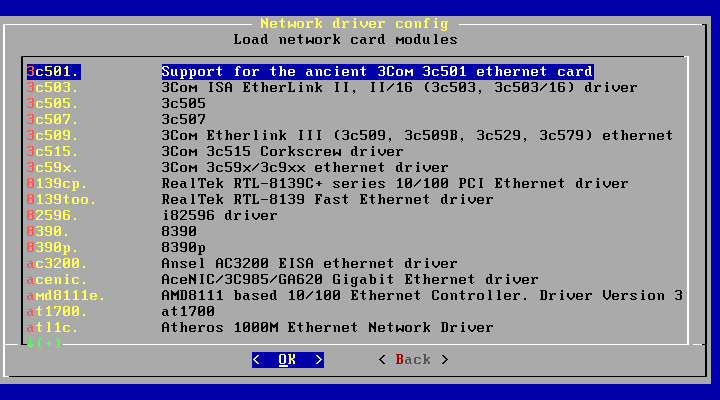
\includegraphics[width=10cm]{img/udpcast_net_module}
\caption{UDP Cast: Selection of the \ac{NIC} Driver}
\label{fig:udpcast_net_module}
\end{figure}



\begin{figure}[h]
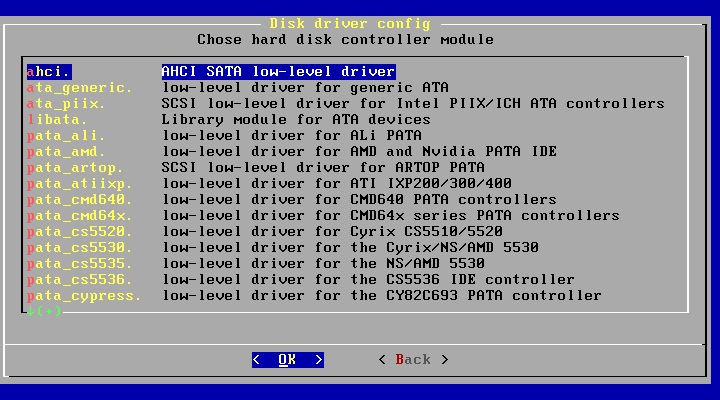
\includegraphics[width=10cm]{img/udpcast_hdd_module}
\caption{UDP Cast: Selection of the \ac{HDD} Driver}
\label{fig:udpcast_hdd_module}
\end{figure}


When the \ac{OS} has loaded the device driver, it can configure
network connectivity. This is done either by setting up a manual IP address
with a valid subnet mask or by use of \ac{DHCP} automatic configuration.
Obtaining an IP address is mandatory for the system to work because,
without an IP, the sender can't connect to the receivers.


\begin{figure}[h]
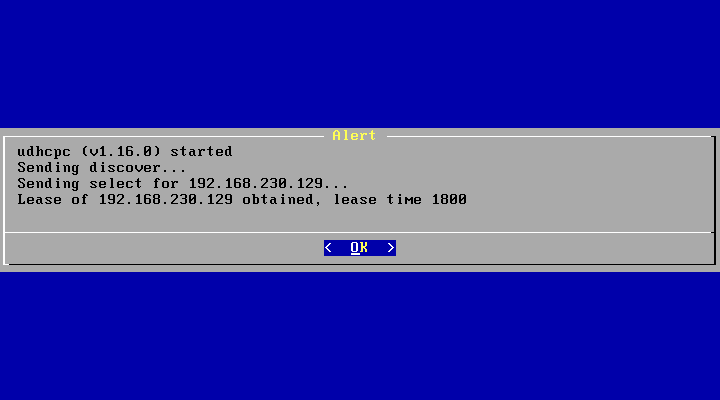
\includegraphics[width=10cm]{img/udpcast_dhcp}
\caption{UDP Cast: Obtaining an IP address via \ac{DHCP}}
\label{fig:udpcast_dhcp}
\end{figure}


After the device driver for the hard disks (PATA, SATA, SCSI) is loaded,
the user must chose what partition or device will be imaged. This has local
significance. On the seed host it will be the partition that will be sent over
the network and on the receivers it will be the partition on which the data
will be written. The name of the partitions are Linux formated. The user
can select a single primary or logical partition (ex. hda1, sda2, sdb5) or
an entire drive (hda, hdb, sda). The \ac{MBR} is found on the first 512bytes of
the physical drive.

It is recommended that the same option be selected on all devices.

\begin{figure}[h]
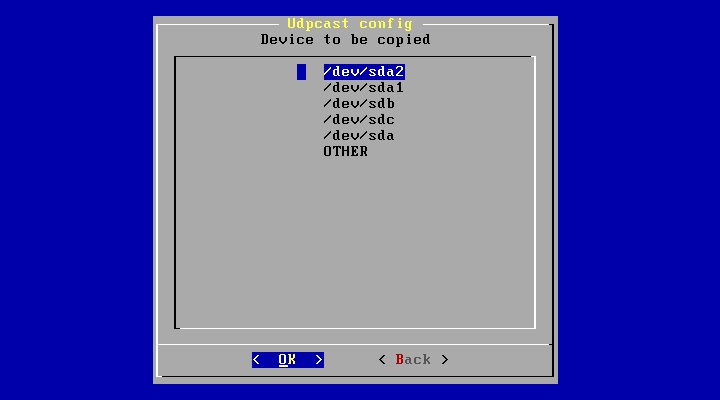
\includegraphics[width=10cm]{img/udpcast_partitions}
\caption{UDP Cast: Selection of the imaged device(physical driver or
partition}
\label{fig:udpcast_partitions}
\end{figure}


A partition is usually has a very large data size and the transfer over the
network could be time consuming. For computers with good enough processing
power, compression can be used. UDP Cast offers two types of compression
\begin{itemize}
\item \ac{LZOP}
\item \ac{GZIP}
\end{itemize}

The use of compression can reduce the sent data by a factor of up to 50\%.

\begin{figure}[h]
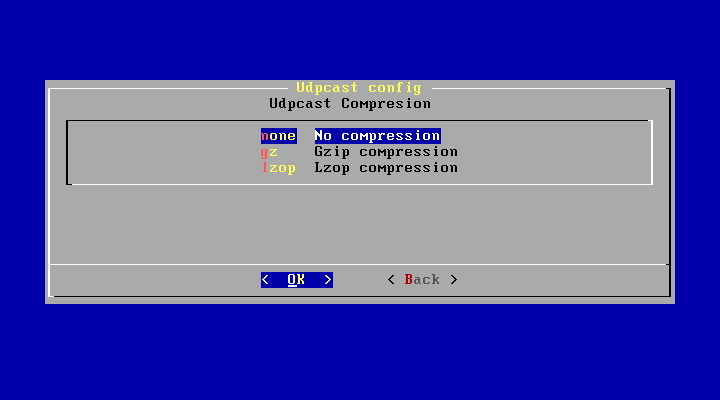
\includegraphics[width=10cm]{img/udpcast_compression}
\caption{UDP Cast: Selection of compression algorithm.}
\label{fig:udpcast_compression}
\end{figure}

After all the configurations are made (they should be identical in most
conditions), the direction of the transfer must be specified on each host.
One workstation will be the sender and all the others will be the
receivers.

\begin{figure}[h]
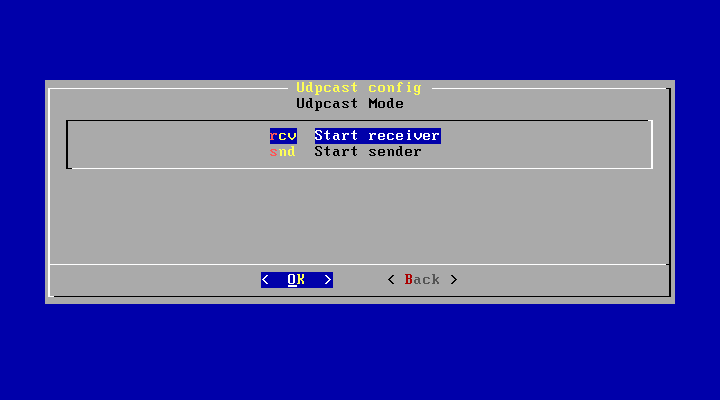
\includegraphics[width=10cm]{img/udpcast_mode}
\caption{UDP Cast: Selection of sender or receiver mode.}
\label{fig:udpcast_mode}
\end{figure}



\section{Multicast}

In the classic client-server model, each connection between a client and
the server is a separate data stream. This means, that if a server has 1000
clients, it needs to open 1000 connections each with it's stream of data.
This is normal, because each connection sends unique data.

But in the case of live streaming (such as audio or video stream) one
server sends the same information to all of it's clients, and using the
classic model, this would mean redundant copied information across the
network. Multicast comes in these kinds of situations and it optimises
the traffic by assuring that the server sends only one data stream and that
data stream is delivered to all of the clients that requested the data.

The imaging data sent during an UDP Cast transfer has the same
characteristics as audios and video streaming so it can be considered live
data, making the use of multicast in the transfer the ideal choice. Unicast
would not scale for the server because if it has more connections it has to
cycle through them all to send something and broadcast would send unwanted
traffic to stations that don't participate in the imaging process.

\subsection{Basics of Multicast}

\cite{cisco:multicast}
\ac{IP} multicast is a bandwidth-conserving technology that
reduces traffic by simultaneously delivering a single stream of information
to thousands of corporate recipients and homes. Applications that take
advantage of multicast include videoconferencing, corporate communications,
distance learning, and distribution of software, stock quotes, and news.

IP Multicast delivers source traffic to multiple receivers without adding
any additional burden on the source or the receivers while using the least
network bandwidth of any competing technology. Multicast packets are
replicated in the network by routers enabled with
\ac{PIM} and other supporting multicast protocols
resulting in the most efficient delivery of data to multiple receivers
possible. All alternatives require the source to send more than one copy of
the data. Some even require the source to send an individual copy to each
receiver. If there are thousands of receivers, even low-bandwidth
applications benefit from using IP Multicast. High-bandwidth
applications, such as MPEG video, may require a large portion of the
available network bandwidth for a single stream. In these applications, the
only way to send to more than one receiver simultaneously is by using IP
Multicast.


\begin{figure}[h]
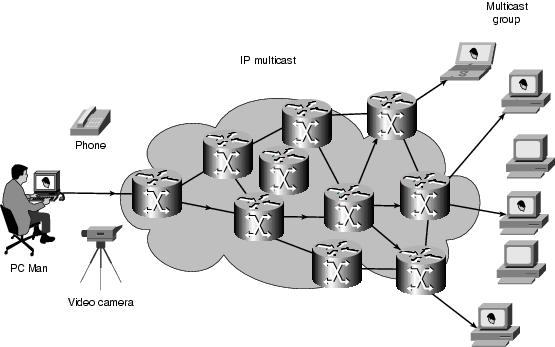
\includegraphics[width=10cm]{img/multicast}
\caption{Multicast Transmission Sending a Single Multicast Packet Addressed
to All Intended Recipients}
\label{fig:multicast}
\end{figure}

\subsection{Multicast Group Concept}

\cite{cisco:multicast}
Multicast is based on the concept of a group. An arbitrary group of
receivers expresses an interest in receiving a particular data stream. This
group does not have any physical or geographical boundaries—the hosts can
be located anywhere on the Internet. Hosts that are interested in receiving
data flowing to a particular group must join the group using \ac{IGMP}.
Hosts must be a member of the group to receive the data stream.


\subsection{IP Multicast Addresses}

\cite{cisco:multicast}
Multicast addresses specify an arbitrary group of IP hosts that have joined
the group and want to receive traffic sent to this group.

The \ac{IANA}  controls the assignment of
IP multicast addresses. It has assigned the old Class D address space to be
used for IP multicast. This means that all IP multicast group addresses
will fall in the range of 224.0.0.0 to 239.255.255.255. 

The \ac{IANA} has reserved addresses in the 224.0.0.0 through 224.0.0.255
to be
used by network protocols on a local network segment. Packets with these
addresses should never be forwarded by a router; they remain local on a
particular LAN segment. They are always transmitted with a time-to-live
(\ac{TTL}) of 1.

\subsubsection{Reserved Link Local Addresses}

\cite{cisco:multicast}
Network protocols use these addresses for automatic router discovery and to
communicate important routing information. For example, OSPF uses 224.0.0.5
and 224.0.0.6 to exchange link state information. 

\begin{table}


\begin{tabular}{| l | r |}
\hline
224.0.0.1 & All systems on this subnet \\
\hline
224.0.0.2 & All routers on this subnet \\
\hline
224.0.0.5 & OSPF routers \\
\hline
224.0.0.6 & OSPF designated routers \\
\hline
224.0.0.12 & DHCP server/relay agent \\
\hline
\end{tabular}
\caption{Multicast Link Local Addresses}
\label{table:multicast_addressed}
\end{table}

\subsubsection{Globally Scoped Address}
\cite{cisco:multicast}
The range of addresses from 224.0.1.0 through 238.255.255.255 are called
globally scoped addresses. They can be used to multicast data between
organizations and across the Internet.

Some of these addresses have been reserved for use by multicast
applications through \ac{IANA}. For example, 224.0.1.1 has been reserved for
\ac{NTP}.

More information about reserved multicast addresses can be found at
http://www.isi.edu/in-notes/iana/assignments/multicast-addresses.


\subsubsection{Limited Scope Addresses}


\cite{cisco:multicast}
The range of addresses from 239.0.0.0 through 239.255.255.255 contains
limited scope addresses or administratively scoped addresses. These are
defined by RFC 2365 to be constrained to a local group or organization.
Routers are typically configured with filters to prevent multicast traffic
in this address range from flowing outside an \ac{AS} or any
user-defined domain. Within an autonomous system or domain, the limited
scope address range can be further subdivided so those local multicast
boundaries can be defined. This also allows for address reuse among these
smaller domains.

\subsubsection{Glop Addressing}
\cite{cisco:multicast}

RFC 2770 proposes that the 233.0.0.0/8 address range be reserved for
statically defined addresses by organizations that already have an AS
number reserved. The AS number of the domain is embedded into the second
and third octets of the 233.0.0.0/8 range.

For example, the AS 62010 is written in hex as F23A. Separating out the two
octets F2 and 3A, we get 242 and 58 in decimal. This would give us a subnet
of 233.242.58.0 that would be globally reserved for AS 62010 to use. 

\subsubsection{Layer 2 Multicast Addresses}

\cite{cisco:multicast}
Normally, \ac{NIC} on a \ac{LAN} segment will receive only
packets destined for their burned-in MAC address or the broadcast MAC
address. Some means had to be devised so that multiple hosts could receive
the same packet and still be capable of differentiating among multicast
groups.

Fortunately, the IEEE \ac{LAN} specifications made provisions for the
transmission of broadcast and/or multicast packets. In the 802.3 standard,
bit 0 of the first octet is used to indicate a broadcast and/or multicast
frame.

\subsubsection{Ethernet MAC Address Mapping}

\cite{cisco:multicast}
The \ac{IANA} owns a block of Ethernet MAC addresses that start with 01:00:5E in
hexadecimal. Half of this block is allocated for multicast addresses. This
creates the range of available Ethernet MAC addresses to be 0100.5e00.0000
through 0100.5e7f.ffff.

This allocation allows for 23 bits in the Ethernet address to correspond to
the IP multicast group address. The mapping places the lower 23 bits of the
IP multicast group address into these available 23 bits in the Ethernet
address.

\subsubsection{Internet Group Management Protocol}

\cite{cisco:multicast}
\ac{IGMP} is used to dynamically register individual hosts in a multicast group
on a particular \ac{LAN}. Hosts identify group memberships by sending
\ac{IGMP}
messages to their local multicast router. Under \ac{IGMP}, routers listen to
\ac{IGMP} messages and periodically send out queries to discover which groups
are active or inactive on a particular subnet.


\subsubsection{Multicast Forwarding}

\cite{cisco:multicast}
In unicast routing, traffic is routed through the network along a single
path from the source to the destination host. A unicast router does not
really care about the source address—it only cares about the destination
address and how to forward the traffic towards that destination. The router
scans through its routing table and then forwards a single copy of the
unicast packet out the correct interface in the direction of the
destination.

In multicast routing, the source is sending traffic to an arbitrary group
of hosts represented by a multicast group address. The multicast router
must determine which direction is upstream (toward the source) and which
direction (or directions) is downstream. If there are multiple downstream
paths, the router replicates the packet and forwards the traffic down the
appropriate downstream paths—which is not necessarily all paths. This
concept of forwarding multicast traffic away from the source, rather than
to the receiver, is called reverse path forwarding. 

\subsubsection{Reverse Path Forwarding}

\cite{cisco:multicast}
\ac{RPF} is a fundamental concept in multicast routing
that enables routers to correctly forward multicast traffic down the
distribution tree. \ac{RPF} makes use of the existing unicast routing table to
determine the upstream and downstream neighbors. A router forwards a
multicast packet only if it is received on the upstream interface. This
\ac{RPF}
check helps to guarantee that the distribution tree will be loop-free. 

\section{UDP over Multicast}

\ac{UDP} is a Transport Layer Protocol in the TCP/IP Stack. The other
protocol at this layer is \ac{TCP}.

The two protocols, TCP and UDP both assure the correct transmission of the
data from a sender process to a receiver process, but the difference is
that TCP is a Reliable Transfer Protocol, while UDP is Best Effort. This
means that TCP guaranties that the data is sent to the destination while
UDP sends the data and hopes it gets safely.

Although TCP is reliable, the transmission of data using TCP has overhead
both in size of the data(larger headers) and in time (TCP needs to have
packets acknowledged). Hence UDP has bigger transmission speeds.

In real lime data streaming (like video, audio streaming), the reliability
of the transmission is not as important as the speed of sending the data.
This makes UDP the normal choice for live data streaming.

Because of how IP Multicast works, UDP is the Transport Layer Protocol of
choice. The sender doesn't need to have the clients acknowledge what it
sends, so reliability is not important. Speed is, because everything has to
real lime.

In UDP Cast, UDP over Multicast is used because of it's speed. This means
that if packets are dropped, at the Transport Layer, they are ignored. But
in an Imaging System, it is not acceptable to have packets ignored because
the packets can be pieces of files. A reliability mechanism has to be in
place, at the Application Layer to ensure that all the data is sent
correctly.

UPC Cast uses ACKs at the Application Layer and a system of timers that
timeout dropped packets so they can be resent.


\section{PXE}


PXE (Preboot eXecution Environment or Pre-Execution
Environment)\cite{wiki:pxe} is a
framework that allows the loading of an Operating System over the network
without having to have any disks on the workstation. It is dependent on
other protocols and concepts such as \ac{IP}, \ac{UDP}, \ac{DHCP} and
\ac{TFTP}.

To boot a system image through \ac{PXE}, you first need to have a workstation
that supports \ac{PXE} in hardware. The Motherboard of the PC must have this
feature and the \ac{BIOS} mush offer the user the option for network boot.

After the chose the network boot, it loads the \ac{PXE} Loader from a ROM on the
Mainboard. This Loader needs to support the whole TCP/IP stack and be able
to start a \ac{DHCP} Client.

The \ac{DHCP} Clients requests an IP address for network connectivity.
For \ac{PXE}
to work, you need to have a server (usually the \ac{DHCP} server) that has a
\ac{TFTP} server that can serve system images. The \ac{DHCP} server passes to the
client along with the IP address and the subnet mask an option (option 200)
for a \ac{TFTP} server.

When the \ac{PXE} enabled client has network connectivity, it can contact the
\ac{TFTP} server and request a system image. The image is downloaded and loaded
into the physical memory of the workstation like a normal \ac{OS}.



\chapter{The Architecture of the System}\label{ch:arch}
\bigskip


\section{The shortcomings of UDP Cast in working environments}

UDP Cast is a tool that saves of time when administering a
large number of workstations in, for example, laboratories for schools. It
is easy do use and customise and does it's rather simple job very
efficient.


Everything with UDP Cast starts with the seed host. This host is the place
where the Operating System (or the multiple Operating Systems) for the host
is installed. All the system updates and the software is installed on this
machine. The UDP Cast Sender will be started on this machine and it will
send all the data to be multiplied on the other hosts. The seed is a host
identical to the other hosts on the network.

\begin{figure}[h]
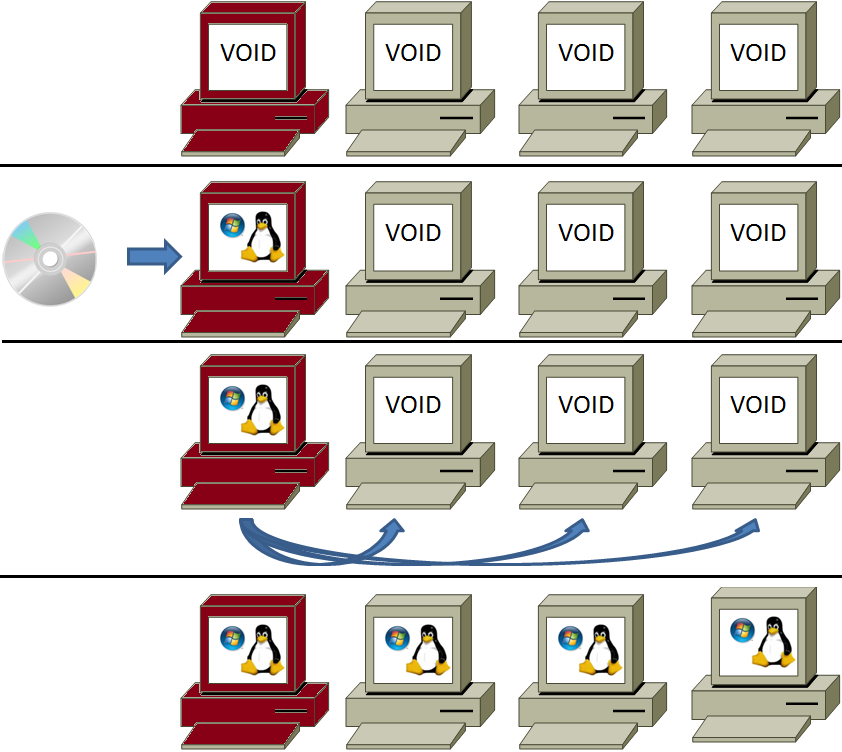
\includegraphics[width=10cm]{img/4comp_seed}
\caption{Seed host (in red)}
\label{fig:s4comp_seed}
\end{figure}

Because of the idea of the seed host being one of the normal hosts in the
network (a decentralised system) certain situations arise where
shortcomings are found. Some of these shortcomings are tried to be resolved
by the subject of this thesis.

\subsection{The Archiving Problem}

After the imaging process, all the hosts should have, at any time, more or
less the same content. The problem is that any old content is lost because
the imaging process means the overwrite of the previous data.

Let us take the example of an University laboratory. Each semester has new
courses with their own labs. Each lab might have different requirements for
the workstations. One lab might use Windows as it's operating system while
the other Linux. One might need an operating system with certain software 
installed while the other other software.

If one laboratory room is used in a year for two courses, one that needs
Setup A and the other Setup B, this means that every semester, an imaging
cycle is needed. This means taking a host, formating it, installing the
required operating system and it's software on it. If Setup A is done at
the beginning of the year, in the second semester, it will be erased and
the next year Setup A will have to be redone.

\subsection{The Backup Problem}

Another situation is where you have a lab with a working operating system
on all computers and a you have a certain lab that specifically asks you to
install an operating system on the host, or modify partitions. This will
cause the radical modification of the hosts and they won't be identical
anymore. Further more some modifications could lead to crashes and render
some hosts useless. The original system would have to be backed up somehow.

One solution is to keep aside one station and after the lab is finished,
use it as a seed to image the other hosts. But this means that you have one
less station to do your lab on.


Another solution is to bring an outside workstation and image it with the
data from the other stations (using one-to-one transfer). This would take
time (because you still need to copy an entire hard disk driver over the
network) and would be logicically hard because you need to bring a station
inside the room and connected with the other ones. Also, the new station
need to have an identical hard drive to receive the data.


\subsection{The Moving Problem}

If you have to image two ore more laboratory rooms (that have the exact
same hardware configuration) with one system image, the two rooms must be
connected to the same network (from a multicast perspective).

If there two rooms are not connected, two things can be done: either do two
separate installs, one in each room, and then run two separate imaging
processes or image in one room and then take one host into the other room
and use it as a seed for the rest of the workstations.

\bigskip

All of the above problems can be resolved by using a centralised system.


\section{The Centralized Approach}

The idea of an imaging system based on UDP Cast is not to rethink what UDP
Cast works or does it's job, but rather to build on top of it and improve
the system and provide and advanced solution for imaging.

The aim of the project is to offer three main features:
\begin{itemize}
\item provide archiving of the system images
\item provide versioning of the system images
\item make a seed server always available and ready to provide images
\end{itemize}

A centralized design requires that a server exists to provide the needed
services. This server will store the system images for all the wanted
setups, each with version history. Clients connect to it and create images
or request archived images. When an images is distributed, the server runs
an udp-sender instance that multicasts the data to the clients.

The server has two main requirements:
\begin{itemize}
\item to be reachable by all the possible clients (eg. all the hosts in all
the laboratory rooms)
\item to have enough storage capacity to hold the images (eg. if you want
to hold up to 3 versions of a system image on a workstation for 40GB of disk
space, you will need at least 120GB of available disk space on the server)
\end{itemize}


\subsection{The Basic Idea}


With this new approach, a new action flow exists, slightly different from
the normal imaging process.


The creation of a system image is still the same. A workstation is cleared
of data, and the needed operating system (or multiple operation systems).
After the setup is done, and the image can be multiplied, the client
program comes in play. Instead of just using the udp-sender to copy data
from the local disk to other disks, it uses a wrapper-client that signals
the Imaging Server that a new image is being created and the Server listens
to a multicast transfer and saves the data locally. The other clients also
receive the image as a normal UDP Cast transfer.


The request for an image is also done via the Client program. One
workstation will have to run the Client to request the image from the
Server. The other clients either start a normal UDP Client, of the Imaging
Clients to receive the image.


To sum up, here are the flow of actions needed:


Image creation:
\begin{itemize}
\item A normal host is prepared with the needed setup. This involves
installing the Operations System(s) and the Software wanted.
\item (Optional) Install the Client locally, as a pseudo operating system,
on a separate partition with a bootloader entry.
\item (Optional) Freeze the system.
\item Launch the Image Client This should be done from a Live Operation
System Environment (or from the locally installed Image Clients as a
separate pseudo operating system, so the installed systems aren't affected.
\item Make a request to the Server to listen for a new image being
transfered.
\item (Optional) Start Image Clients or UDP Cast clients on other
workstations receive the image.
\item Start the transfer.

\end{itemize}
Image request:
\begin{itemize}
\item Start the Image Client on a workstation.
\item Send an Image Request to the Image Server for version of a system
image.
\item Start Clients on the workstations that will be imaged.
\item Start the transfer.
\end{itemize}

\subsection{The Network Boot Server}

The Image Client and the UDP Cast Client should boot from a non-used
operating system, like a Live CD or a network boot. It can either be
installed local as a separate \ac{OS} (different partition) or just as a
separate kernel (using an existing partition) as long as it has a valid
bootloader entry.

Another possibility is to have it as Network Boot Image. This way, as long
as the workstation is connected to the network, it can always boot this
image.

The Network Boot Image requires a PXE Server and the workstations need to
have hardware that supports \ac{PXE} Network Boot. The \ac{DHCP} Server for the local
network need to give out to the hosts the \ac{TFTP} server option so the hosts
can get the image from the \ac{TFTP} Server. The \ac{TFTP} Server will be on the same
machine as the Image Server and have special image with the Image Client.
This image will be a simple linux based distribution.


\section{The Choice of a Framework}

The described architecture can be implemented in verious ways. Some of the
considered were:
\begin{itemize}
\item C and different network libreries
\item Bash and the core-utils programs found in GNU/Linux distributions
\item Python
\item combinations of C, Bash and Python
\end{itemize}

\cite{wiki:python}
Python is a general-purpose high-level programming language whose
design philosophy emphasizes code readability.  Python aims to combine
"remarkable power with very clear syntax",  and its standard library is
large and comprehensive. Its use of indentation  for block delimiters is
unusual among popular programming languages.

Python supports multiple programming paradigms, primarily but not limited
to object oriented, imperative and, to a lesser extent, functional
programming styles. It features a fully dynamic type system and automatic
memory management, similar to that of Scheme, Ruby, Perl, and Tcl. Like
other dynamic languages, Python is often used as a scripting language, but
is also used in a wide range of non-scripting contexts.

The reference implementation of Python (CPython) is free and open source
software and has a community-based development model, as do all or nearly
all of its alternative implementations. CPython is managed by the
non-profit Python Software Foundation.

The choice was Python for 3 main reasons:
\begin{itemize}
\item easier to code compared to C
\item large number of libraries
\item portable to many operating systems
%\item it is open source
\end{itemize}



\chapter{The Imaging Client}\label{ch:client}

The client is represented by the \emph{client.py} Python script. The
requirements for running it are:
\begin{itemize}
\item the Python interpreter installed (multi platform)
\item the UDP Cast udp-sender and udp-receiver installed
\end{itemize}

There are several possibilities or running an Imaging Client:
\begin{enumerate}
\item from a locally installed operating system
\item from a separate partition on the local system
\item from a network boot image
\end{enumerate}

The first one is not recommended because if you want to copy the image of
the running operating system, it's contents might change during the
transfer and will invalidate the image.

A network boot should be the best option, because a server is already in
place and could be setup to service a \ac{PXE} image that contains the script.

The Image Client has a command line interface that accepts the commands
supported.

\begin{lstlisting}[caption= Image Client CLI]
**************************************
*Welcome to the Imaging System Client*
**************************************

Available commands:
l: list images on servers
c: create image
u: update image
d: delete image
r: request image
>>
\end{lstlisting}

Each command sends a request to the Image Server to execute an action.


\section{Image listing}

The first command is a request for the server to list the stored images in
the database. The client sends a "LIST" request and waits for the answer.

If the server receives a "LIST" request, it explores the \emph{images}
directory and it's contents. Each directory represents the ID of a system
image. In each ID-directory the is a \emph{info} file that contains the
description and a directory for each disk/partition in the image. Each
partition or disk directory has one or more directories that contain a
version of that image-disk.

Based on the information in the \emph{file} and the structure of the
directory hierarchy, the server sends a reply to the clients with the
needed information. The Client then displays the information to the user.

\section{Image Creation}

The creation of an image involves work both on the client and on the
server. 

When an image in created, the Image Client must be ran on the workstation
that contains the operating system(s) that will be imaged on the other
hosts. The client will scan the workstation for disks and partition.

A command line wizard will be started and the user will have to enter a
description for the image.

\begin{lstlisting}[caption=Image creation wizard on Image Client]
Available commands:
l: list images on servers
c: create image
u: update image
d: delete image
r: request image
>>c
 Creating image...
Available disks:
* sda
   - sda5
   - sda2
   - sda1
Fill in description for the image (press CTRL-D to finish reading input)
Image for room EG306-USO (Ubuntu 10.4 Customised)
Start transfer to server (it might take a long time)?[y/n]

\end{lstlisting}

The search for the devices is done using the \emph{/dev} system directory
in Linux.


\begin{lstlisting}[float, caption=Code snip of device listing]
def create_image():
	print "Creating image..."

	# Searching local disks and partitions 
	disks =  filter(re.compile("[sh]d.$").search, os.listdir("/dev"))
	print "Available disks:"
	for disk in disks:
		print "*", disk
		partitions =  filter(re.compile(disk + ".+$").search,
os.listdir("/dev"))
		for partition in partitions:
			print "   -", partition
\end{lstlisting}

This information is sent to the server that prepares a new ID for the
image. It will be considered version 1 of this image. The description is
stored in the \emph{info} file on the server in the corresponding directory.

After the devices to be copied are chosen, the client signals the server to
start an udp-receiver process to listen for the data. After the server has
started the process, the client start a local udp-sender with the input
being the selected partition(s).

At this point, on other workstations, Image Clients in request image mode
or normal UDP Cast clients can be started to also receive the image. This
saves time by both imaging all the hosts and archiving the image on the
server.

When all the receivers are connected, the transfer is started.

\section{Image Update}

Once an image for a workstation is on the server in an initial version, new
versions of a disk or a partition can be uploaded to the server. The
operation is similar to the creation, only the server does not create a new
ID, but only listens to new data images to be stored in the same directory
hierarchy.

\section{Image Deletion}

To free up space on the server old images can be deleted. The user can either
delete an entire image entry or just a version of a disk or a partition.

\section{Image Request}

The image request operation is similar to what UDP Cast does as a receiver.
A request for an image ID is send to the server, that starts a udp-sender
process with the selected version of a disk or partition.

All the workstations that need to be imaged, need to run the Image Client
in Image Request mode or run the UDP Cast receiver.



\chapter{The Imaging Server}\label{ch:server}

Like the client, the server is a Python script called  \emph{server.py}.
The main purpose of the server is to store the images created on the
workstations in the network. For this, it used a hierarchy in the file
system that stores images in binary files, with meta information in
other files.

All the images are stored in the \emph{images/} directory. For each image
there is an unique ID with a corresponding directory with the ID as the
name. In each ID-directory the is a \emph{info} file that contains the
description and a directory for each disk/partition in the image. Each
partition or disk directory has one or more directories that contain a
version of that image-disk.

\begin{lstlisting}[caption= Images directory hierarchy on the Image Server]
images/
|-- 1
|   |-- info
|   |-- sda
|   |   |-- 1
|   |   |-- 2
|   |   `-- 3
|   `-- sdb
|       `-- 1
|-- 10
|   `-- info
|-- 11
|   `-- info
|-- 12
|   `-- info
|-- 2
|   |-- info
|   `-- sda
|       |-- 1
|       |-- 2
|       |-- 3
|       |-- 4
|       `-- 5
|-- 3
|   |-- info
|   |-- sda1
|   |   `-- 1
|   `-- sda5
|       `-- 1
`-- 5
    `-- info

\end{lstlisting}

The Image Server awaits connections from clients. Because only one image
can be transfered at a time, only one client can connect at a time.

From the clients, the following requests can be received:
\begin{itemize}
\item LIST
\item CREATE
\item UPDATE
\item DELETE
\item REQUEST
\end{itemize}

The LIST actions is a request to send to the client information about the
images in the server's image database. The request can either be sent with
a value of 0, in which case the server will send information on all the
images, or with a value that is an ID of an image, in which case, only
information about the specified image is sent back to the client.

The CREATE, UPDATE and DELETE actions involve modifying  the image
database. CREATE will make a new image with a new ID and a directory in the
\emph{images/} directory, with a base version 1, while UPDATE will only
create a new version of a partition or disk in an existing image. DELETE
will erase an image.

In the case of CREATE and UPDATE, the client will ask the server to start a
udp-receiver process. The client has a udp-sender process started. When the
client gives the command, the server will receive the data and store the
sent partition or disk image in the local database.

When a REQUEST command is sent, the server will provide via a udp-sender
instance the content of a partition or disk to the upd-sender clients in
the network.



\chapter{Conclusions and Future Development}\label{ch:conclusions}


The implementation of the project offers new features to the UDP Cast
framework, making is better suited for environments such as School and
University Computer Laboratories.

The main benefit of using the proposed architecture for system imaging is
the time saved in various situations. The costs of implementing such a
system is very small so it is appealing to be used.

The current version of the software implements the idea of a centralised
system in a very basic way. Some of the current shortcomings, that can be
mended in future development include:

\begin{itemize}
\item The Server can only serve one client at a time. This is because of
the way UDP Cast works, because it was designed to have one transfer at a
time. A modified implementation could make the server have udp-senders on
multiple multicast addresses and by keeping track of the source address,
more then one transfer could be made. This could lead to some
synchronisation problems on the image database and since the resources in
the archive are large files, locking could be an issue.
\item The client to server requests are done without authentication. Anyone
with a client can connect to the sever and add, remove and modify images.
This could be secured by creating a database of users (with different
privilege levels) and make the server ask for credentials before receiving
any requests from clients. Furthermore, the use of SSL/TLS could make the
control traffic immune to traffic sniffing.
\item The Client only offers a \ac{CLI} for sending requests to the sever and
doing any actions. A \ac{GUI} could provide a more user friendly
environment for users.
\item New versions of an image means copying new files to the server. These
files are very big in size (10-100GB) and could easily occupy the server's
disk space. A differential versioning system could reduce the file sizes by
making version 1 a base version and only storing the differences between
the base version and the new version on the server's disk.
\end{itemize}




%\addtocontents{toc}{\protect\clearpage} % <--- just debug stuff, ignore
%\include{multiToC} % <--- just debug stuff, ignore for your documents
% ********************************************************************
% Backmatter
%*******************************************************
\appendix
\cleardoublepage%\part{Appendix}
%\include{chapters/Chapter0A}
%********************************************************************
% Other Stuff in the Back
%*******************************************************
\cleardoublepage%********************************************************************
% Bibliography
%*******************************************************
% work-around to have small caps also here in the headline
\manualmark
\markboth{\spacedlowsmallcaps{\bibname}}{\spacedlowsmallcaps{\bibname}} % work-around to have small caps also
%\phantomsection 
\refstepcounter{dummy}
\addtocontents{toc}{\protect\vspace{\beforebibskip}} % to have the bib a bit from the rest in the toc
\addcontentsline{toc}{chapter}{\tocEntry{\bibname}}
\bibliographystyle{plainnat}
\label{app:bibliography}
\bibliography{bibliography}

%\cleardoublepage\pagestyle{empty}

\hfill

\vfill


\pdfbookmark[0]{Colophon}{colophon}
\section*{Colophon}
This thesis was typeset with \LaTeXe\ using Hermann Zapf's
\emph{Palatino}
and \emph{Euler} type faces (Type~1 PostScript fonts \emph{URW
Palladio L}
and \emph{FPL} were used). The listings are typeset in \emph{Bera
Mono}, originally developed by Bitstream, Inc. as ``Bitstream Vera''.
(Type~1 PostScript fonts were made available by Malte Rosenau and
Ulrich Dirr.)

The typographic style was inspired by \cauthor{bringhurst:2002}'s genius as
presented in \emph{The Elements of Typographic Style} 
\citep{bringhurst:2002}. It is available for \LaTeX\ via \textsmaller{CTAN} as 
``\href{http://www.ctan.org/tex-archive/macros/latex/contrib/classicthesis/}%
{\texttt{classicthesis}}''.

\paragraph{note:} The custom size of the textblock was calculated
using the directions given by Mr. Bringhurst (pages 26--29 and
175/176). 10~pt Palatino needs  133.21~pt for the string
``abcdefghijklmnopqrstuvwxyz''. This yields a good line length between
24--26~pc (288--312~pt). Using a ``\emph{double square textblock}''
with a 1:2 ratio this results in a textblock of 312:624~pt (which
includes the headline in this design). A good alternative would be the
``\emph{golden section textblock}'' with a ratio of 1:1.62, here
312:505.44~pt. For comparison, \texttt{DIV9} of the \texttt{typearea}
package results in a line length of 389~pt (32.4~pc), which is by far
too long. However, this information will only be of interest for
hardcore pseudo-typographers like me.%

To make your own calculations, use the following commands and look up
the corresponding lengths in the book:
\begin{verbatim}
    \settowidth{\abcd}{abcdefghijklmnopqrstuvwxyz}
    \the\abcd\ % prints the value of the length
\end{verbatim}
Please see the file \texttt{classicthesis.sty} for some precalculated 
values for Palatino and Minion.

    \settowidth{\abcd}{abcdefghijklmnopqrstuvwxyz}
    \the\abcd\ % prints the value of the length


\bigskip

\noindent\finalVersionString




%\cleardoublepage%*******************************************************
% Declaration
%*******************************************************
\refstepcounter{dummy}
\pdfbookmark[0]{Declaration}{declaration}
\chapter*{Declaration}
\thispagestyle{empty}
Put your declaration here.
\bigskip
 
\noindent\textit{\myLocation, \myTime}

\smallskip

\begin{flushright}
    \begin{tabular}{m{5cm}}
        \\ \hline
        \centering\myName \\
    \end{tabular}
\end{flushright}

% ********************************************************************
% Game Over: Restart, Restore or Quit?
%*******************************************************
\end{document}
% ********************************************************************
